%!TEX root = main.tex
%%%%%%%%%%%%%%%%%%%%%%%%%%%%%%%%%%%%%%%%%%%%%%%%%%%%%%%%%%%%%%%%%%%%%%%%%%%%%%%%

\section{Results}
\label{sec:results}

\begin{figure}[t]
\centering
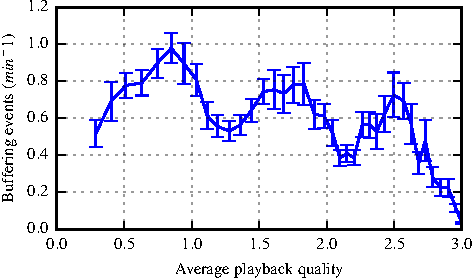
\includegraphics[width=0.95\linewidth]{figs/33qualityvstalling}%
\caption{Average playback quality versus stalling events}
\label{fig:qualityvsstalling}%
\end{figure}

Figure \ref{fig:qualityvsstalling} illustrates the relationship between the average quality level and the stalling events in the experiment result set.
For the average quality level, 0 is defined as \unit[100]{\%} of the segments are shown to the user in 144p. 3 is defined as \unit[100]{\%} of the segments are shown to the user in 480p.
The average quality levels are clustered using k-means and the error bars indicate the \unit[95]{\%} confidence interval of each cluster.
Two observations can be made from the figure. First, the lowest average quality level is 0.3 with about 0.5 switches per minute.
From this it follows that the player risks one stalling per two minutes in order to not constantly show the lowest quality level in low bandwidth scenarios.
Second, the buffering events exhibit an oscillating behavior.
The oscillating behavior is consistent with observations made in \cite{sieber16sacrificing}.
The study shows that the behavior of YouTube's adaptation algorithm depends on the relationship between video bit-rate and available bandwidth.


pearson correlation -0.773713

\subsection{optimal adaptation}

Idea: calculate the highest resolution that could have been achieved. compare it to measurement data. How much can still be gained?
opt was calculated according to the optimization problem in \cite{hossfeld2015identifying}. The calculations were done using the Gurobi Optimizer\footnote{http://www.gurobi.com/}.

In total we have four sets of results that we compare to each other:
\begin{itemize}
\item \textit{measurement}: the originally measured data set from \cite{sieber16sacrificing}; notice that stalling occured in these runs
\item \textit{opt (regression)}: assume that each segment is only downloaded once; same amount of stalling as measurement; was calculated in \cite{sieber16sacrificing}
\item \textit{opt (same stalling as measurement)}: gurobi (optimize mean quality based on \cite{hossfeld2015identifying}); same amount of stalling as measurement
\item \textit{opt (no stalling)}: gurobi (optimize mean quality based on \cite{hossfeld2015identifying}); no stalling
\end{itemize}

\begin{figure}[t]
\centering
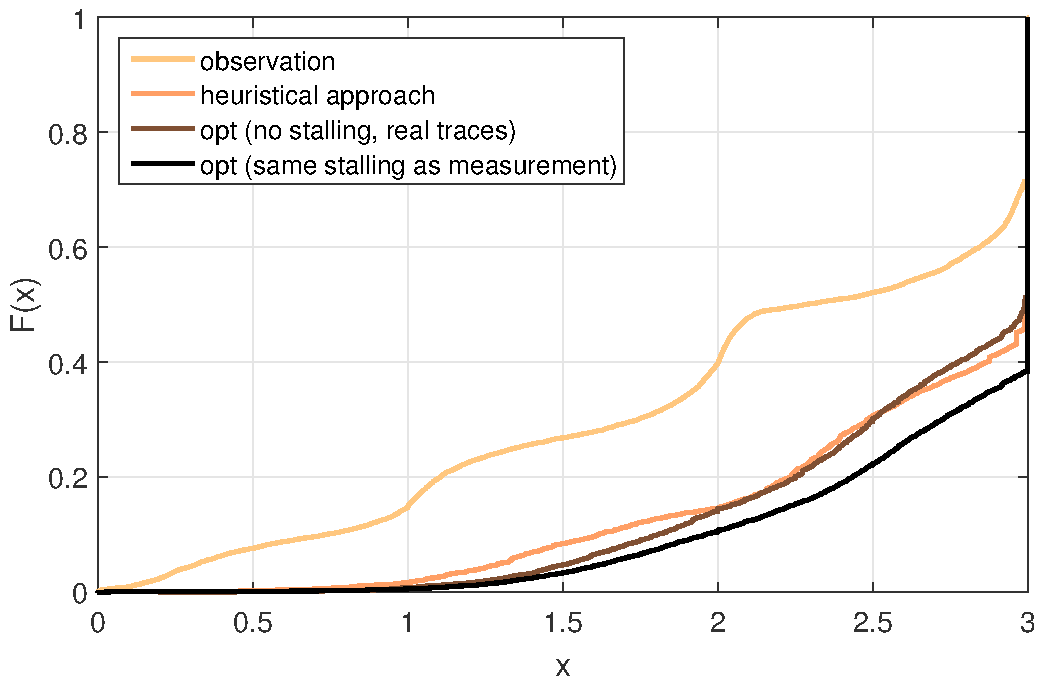
\includegraphics[width=0.5\textwidth]{figs/quality}%
\caption{CDF of the mean video quality in the measurement runs and highest achievable mean video quality according to the optimization problem in \cite{hossfeld2015identifying}. Remake figure!}
\label{fig:opt}%
\end{figure}

\begin{figure}[t]
\centering
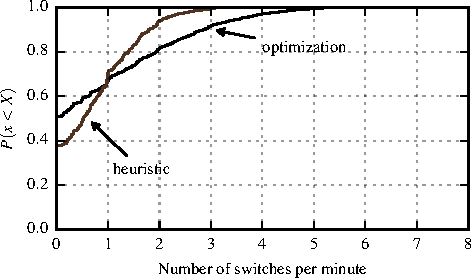
\includegraphics[width=0.5\textwidth]{figs/switches}%
\caption{CDF of the number of switches per minute. Remake figure!}
\label{fig:switches}%
\end{figure}

In figure \ref{fig:opt} we see the CDF of the mean video quality in the measurement runs and highest achievable mean video quality according to the optimization problem. In addition, we added an estimation of the avg. quality level that is possible based on downloaded data that was done in \cite{sieber16sacrificing}. While stalling events occured frequently during the original measurement, stalling events are not allowed to occur in the optimization problem. Therefore, we consider two sets of input for the opt. prob. for each measurement run: First, we only consider the available bandwidth during the video download. Second, we also respect the stalling events that occured. The sum of stalling was then added as initial delay during which the video was downloaded. In contrast to the YouTube measurement data where the video buffer does not contain more than 50s of video content at a time, in the calculations of the optimal adaptation we assumed that the video buffer is not limited.
